\section{Camada Lógica}

A camada lógica, também designada por camada de negócios, situa-se na posição intermédia no modelo de três camadas abordado e estudado neste relatório.
Analisando este modelo sobre uma perspetiva \textit{bottom-up}, a camada de negócios (\textit{layer II}) surge depois da camada de dados (\textit{layer I})e é sucedida pela camada apresentacional (\textit{layer III}).\\

O \textit{software} desenvolvido para esta camada é executado, apenas e só, no servidor da aplicação.
Num modelo de desenvolvimento de uma aplicação seguindo o modelo de três camadas, é esperado que a camada lógica assegure os seguinte objetivos:

\begin{itemize}

\item
Definição das Classes do Problema

\item
Definição da Lógica Aplicacional

\item
Validação das Regras de Negócio

\end{itemize}

Como referido no primeiro ponto, o desenho da solução do problema ocorre, quase por exclusivo, nesta camada.
Assim, e uma vez que estamos num ambiente de programação orientada aos objetos, e, em particular, recorrendo à linguagem \textit{Java}, é nesta camada que serão desenvolvidas os \textit{packages} e as classes que representam as entidades do domínio do problema.
É também nestas classes que estará explícita as regras de negócio constituintes da aplicação e onde também será feita as validações ao modelo adotado.\\

O facto desta camada ser a camada intermédia faz com que desempenhe também um papel fundamental na comunicação entre as outras duas camadas.
Assim, a camada de negócios é responsável por receber e processar os pedidos que a camada de interface com o utilizador lhe faz chegar e, por sua vez, comunicar com a camada de dados caso seja necessária atualizar o estado da aplicação.\\

\begin{figure}[!h]
\centering
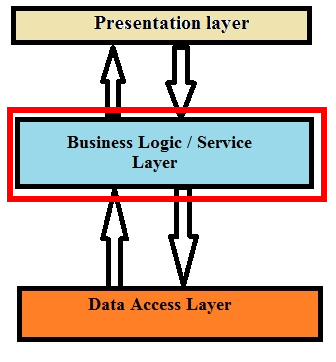
\includegraphics[scale=.4]{img/camada-logica}
\caption{Modelo das três camadas com enfâse na camada lógica}
\end{figure}

Devido a esta interoperabilidade permanente, facilmente se verifica que esta camada arcará com a maior parte do processamento da aplicação, pelo que otimizações ao código desenvolvido para resultam, em grande parte das vezes, num ganho significativo a nível de \textit{performance} da aplicação.\\

Pode-se então afirmar, com certeza, que é nesta \textit{Business Layer} que se encontra o \textit{core} da aplicação.\\

Importa agora enquadrar as \textit{frameworks} no contexto da camada que está a ser analisada.
As \textit{frameworks} surgem com o objetivo de, essencialmente, facilitar o processo de desenvolvimento de \textit{software} e, assim, tornar mais eficiente e produtivo a produção da aplicação.
Estas permitem ao programador trabalhar a um nível mais alto de abstração, automatizando, e por forma a fornecer um exemplo, o processo de \textit{queries} à base de dados, que, como se sabe, é uma tarefa algo repetitiva.\\

Para a análise comparativa destas ferramentas para a camada de negócio foram selecionadas duas \textit{frameworks}: \textit{\textbf{Enterprise JavaBeans}} e \textit{\textbf{Spring}}.
O estudo de comparação assentará em critérios como \textit{(i)} o tempo necessário para dominar a ferramenta, \textit{(ii)} a portabilidade, \textit{(iii)} a integração de testes unitários e \textit{(iv)} a documentação disponível fornecida tanto por fonte oficial como pela comunidade.

\subsection{\textit{Enterprise JavaBeans Technology}}

A \textit{Enterprise JavaBeans}, também conhecida como \textit{EJB}, é uma \textit{framework} responsável pela encapsulamento da componente, por parte do servidor, da lógica de negócio de uma dada aplicação.
A especificação original foi inicialmente desenvolvida pela \textit{IBM}, sendo adotada, mais tarde, pela \textit{Sun Microsystems}.
Desde então, esta especificação tem sido mantida e melhorada pelo formalismo \textit{Java Community Process}.\\

O objetivo desta tecnologia é colocar ao dispôr do programador uma forma standardizada de desenvolver a lógica de \textit{back-end} de uma aplicação \textit{web}.
Este desenvolvimento é feito num nível mais alto de abstração, uma vez que é a própria \textit{framework} que se encarrega das tarefas como a persistência da informação na base de dados, a garantia de integridade das transações e da segurança, permitindo que a equipa de desenlvovimento se foque na arquiterua desenvolvida para dar resposta ao problema e na lógica de negócio associada.\\

\begin{figure}[!h]
\centering
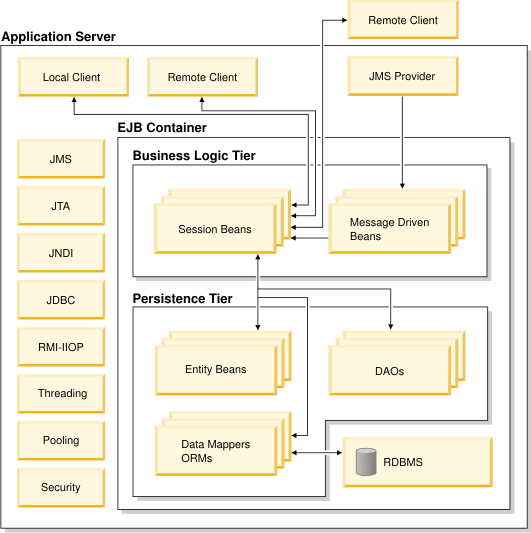
\includegraphics[scale=.4]{img/ejb}
\caption{Arquitetura do \textit{EJB}}
\end{figure}

No que se refere aos critérios de comparação, e começando no tempo que será necessário dispender para dominar a ferramenta, consta-se que pelo facto de fazer parte do standards de \textit{Java} torna o processo adpatativo bem mais curto.
Qualquer programador de \textit{Java} se sentirá familiar com a forma como a \textit{API} foi organizada e desenvolvida.\\

\newpage

Relativamente à portabilidade desta \textit{framework}, e por se tratar de \textit{software} produzido para a \textit{Java Virtual Machine}, esta ferramenta deverá ser, à partida, independente da plataforma, significando, portanto, que poderá ser executada em qualquer conjunto de \textit{Hardware+Software} onde a máquina virtual do \textit{Java} seja suportada, o que, atualmente, acontece com a grande parte dos computadores e dispositivos móveis.\\

Já quanto à realização de testes unitários, esta é possível e é feita através do módulo de \textit{JUnitEE}.\\

Por último, importa fazer um comentário acerca da documentação existente para esta \textit{framework}.
Ora, como é do conhecimento geral, um dos pontes fortes do \textit{Java} é a sua detalhada documentação e, sendo este um standard que é parte constituinte da linguagem, a documentação existente é bastante satisfatória.
A comunidade também desempenha um papel importante na hora de adoção a uma \textit{framework} e a desta, incorporada na de Java, também não desilude.
Desta forma, não deverá ser difícil encontrar apoio \textit{online} para questões relacionadas com esta tecnologia.

\subsection{\textit{Spring Framework}}

A \textit{framework Spring} é outra solução a ter em conta no âmbito de desenvolvimento de \textit{software} para a camada de negócios.
Esta tem como objetivo lidar da infraestrutura e do servidor aplicacional onde a aplicação é executada, fazendo com que a equipa de desenvolvimento se possa focar primariamente no desenho da arquitetura que visa dar resposta ao problema.\\

O \textit{Spring} apresenta-se como um framework perfeitamente modular.
É composta, assim, por várias componentes e dá total liberdade de escolha ao programador para integrar os módulos que são necessários para a especificidade do problema.
A \textit{big picture} da arquitetura do Spring, com todos os seus módulos, é apresentada na figura seguinte.\\

\begin{figure}[!h]
\centering
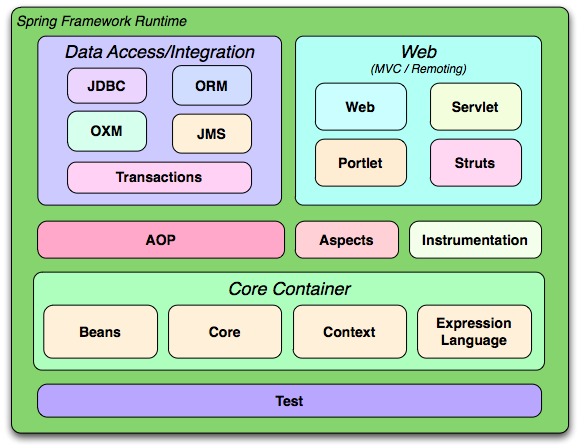
\includegraphics[scale=.4]{img/spring}
\caption{Arquitetura da \textit{Spring Framework}}
\end{figure}

Das componentes exibidas na figura anterior, apenas são relevantes para este caso de estudo as pertencentes ao módulo \textit{Core Container}.\\

Efetuando uma pequena análise à facilidade ou não de aprendizagem desta tecnologia, verifica-se que, apesar do vasto leque de recursos existentes, ainda é necessário um tempo de adaptação razoável para lidar com esta \textit{framework}.\\

A portabilidade não aparenta ser um problema, já que esta corre em cima da máquina virtual do \textit{Java}.\\

Esta \textit{framework} revela preocupação e incentiva à realização e utilização de testes unitários às aplicações desenvolvidas com esta.
Os testes podem também ser do tipo de integração, onde são verificadas e validadas as informações da cache e as meta-anotações presentes nas classes desenvolvidas para a solução do problema.\\

A documentação da \textit{framework} está bem organizada e são cobertos todos os tópicos.
Ao nível da comunidade, o fórum oficial desta ferramenta será a melhor forma para obter respostas a eventuais dúvidas que possam aparecer.

\subsection{Comparação Final}

As duas \textit{frameworks} apresentadas revelam-se como soluções sólidas, robustas e escaláveis para o desenvolvimento da camada de negócios aplicacional.\\

No entanto, e havendo a necessidade de se efetuar uma escolha, a opção recai no \textit{EJB}, dado que, por um lado, é um standard do Java e, por outro, apresenta uma comunidade bem maior do que a existente em Spring.
Na portabilidade, o \textit{EJB} também se destaca pelas garantias mais seguras de portabilidade comparativamente ao \textit{Spring}.
